\documentclass{beamer}
\mode<presentation>

%% packages
\usepackage{beamerthemeshadow}
\usepackage{xcolor}
\usepackage[english]{babel}
\usepackage[latin1]{inputenc}
\usepackage{times}
\usepackage[T1]{fontenc}
\usepackage{wrapfig}
\usepackage{color}
\usepackage{graphicx}
\usepackage{subfigure}
\usepackage{multirow}
\usepackage{amsmath}
\usepackage{tikz}
\usetikzlibrary{automata,positioning,arrows}
\usepackage{tikz,ifthen}
\usepackage{etoolbox}
\usepackage{hyperref}

%% The Beamer class comes with a number of default slide themes which change the colors and layouts of slides. For more details go to  http://deic.uab.es/~iblanes/beamer_gallery/
%\usetheme{default}
%\usetheme{AnnArbor} % Yellow colored theme, 3 parition in footer
%\usetheme{Antibes}  % Blue shadowed theme, 2 partition in footer
%\usetheme{Bergen}   % left side navigation, 2 partition in footer
%\usetheme{Berkeley}
%\usetheme{Berlin}   % bottom vertical partition, horizontal top navigation
%\usetheme{Boadilla} % light blue navigation, 3 partition at bottom
%\usetheme{CambridgeUS} % red color cool theme, 3 partition
%\usetheme{Copenhagen}
%\usetheme{Darmstadt}
%\usetheme{Dresden}
\usetheme{EastLansing} % cool green colored theme
%\usetheme{Frankfurt}
%\usetheme{Goettingen}
%\usetheme{Hannover}
%\usetheme{Ilmenau}
%\usetheme{JuanLesPins}
%\usetheme{Luebeck}
%\usetheme{Madrid}
%\usetheme{Malmoe}
%\usetheme{Marburg}
%\usetheme{Montpellier}
%\usetheme{PaloAlto}
%\usetheme{Pittsburgh}
%\usetheme{Rochester}
%\usetheme{Singapore}
%\usetheme{Szeged}
%\usetheme{Warsaw}

%% As well as themes, the Beamer class has a number of color themes for any slide theme.
%\usecolortheme{albatross}
%\usecolortheme{beaver}
%\usecolortheme{beetle}
%\usecolortheme{crane}
%\usecolortheme{dolphin}
%\usecolortheme{dove}
%\usecolortheme{fly}
%\usecolortheme{lily}
%\usecolortheme{orchid}
%\usecolortheme{rose}
%\usecolortheme{seagull}
%\usecolortheme{seahorse}
%\usecolortheme{whale}
%\usecolortheme{wolverine}

%% font themes
%\usefonttheme{structurebold}
%\usefonttheme{professionalfonts}
%\usefonttheme{structuresmallcapsserif}
%\usefonttheme{serif}
\usefonttheme{structureitalicserif}

%% color definition
\definecolor{theme_color}{RGB}{0,51,25}

%% custom color
%\setbeamercolor{alerted text}{fg=orange}
%\setbeamercolor{background canvas}{bg=white}
%\setbeamercolor{block body alerted}{bg=normal text.bg!90!black}
%\setbeamercolor{block body}{bg=normal text.bg!90!black}
%\setbeamercolor{block body example}{bg=normal text.bg!90!black}
%\setbeamercolor{block title alerted}{use={normal text,alerted text},fg=alerted text.fg!75!normal text.fg,bg=normal text.bg!75!black}
%\setbeamercolor{block title}{bg=blue}
%\setbeamercolor{block title example}{use={normal text,example text},fg=example text.fg!75!normal text.fg,bg=normal text.bg!75!black}
%\setbeamercolor{fine separation line}{}
%\setbeamercolor{frametitle}{fg=brown}
%\setbeamercolor{item projected}{fg=black}
%\setbeamercolor{normal text}{bg=black,fg=yellow}
%\setbeamercolor{palette sidebar primary}{use=normal text,fg=normal text.fg}
%\setbeamercolor{palette sidebar quaternary}{use=structure,fg=structure.fg}
%\setbeamercolor{palette sidebar secondary}{use=structure,fg=structure.fg}
%\setbeamercolor{palette sidebar tertiary}{use=normal text,fg=normal text.fg}
%\setbeamercolor{section in sidebar}{fg=brown}
%\setbeamercolor{section in sidebar shaded}{fg= grey}
%\setbeamercolor{separation line}{}
%\setbeamercolor{sidebar}{bg=red}
%\setbeamercolor{sidebar}{parent=palette primary}
\setbeamercolor{structure}{fg=theme_color}
%\setbeamercolor{subsection in sidebar}{fg=brown}
%\setbeamercolor{subsection in sidebar shaded}{fg= grey}
%\setbeamercolor{title}{fg=brown}
%\setbeamercolor{titlelike}{fg=brown}

%% control header
\setbeamertemplate{headline}{}

%% control footer
%\setbeamertemplate{footline}
%\setbeamertemplate{footline}[page number]

%% removes navigation symbol
%\setbeamertemplate{navigation symbols}{}

%% bibilography settings
\setbeamertemplate{frametitle continuation}[from second]
\setbeamercolor*{bibliography entry title}{fg=black}
\setbeamercolor*{bibliography entry author}{fg=black}
\setbeamercolor*{bibliography entry location}{fg=black}
\setbeamercolor*{bibliography entry note}{fg=black}

%% same slide number for continuation slides
\newcounter{multipleslide}
\makeatletter
\newcommand{\multipleframe}
{
	\setcounter{multipleslide}{\value{framenumber}}
	\stepcounter{multipleslide}
	\patchcmd{\beamer@@tmpl@footline}
	{\insertframenumber}
	{\themultipleslide}
	{}
	{}
}
\newcommand{\restoreframe}
{
	\patchcmd{\beamer@@tmpl@footline}
	{\themultipleslide}
  	{\insertframenumber}
	{}
	{}
	\setcounter{framenumber}{\value{multipleslide}}
}
\makeatother

%% title page
\title[Dynamic Server Consolidation (simcon)]
{
	R \& D Project (CS 490) \\
	Dynamic Server Consolidation Problem \\
	as Markov Decision Process
}
\author[Aman Mangal, Amit Panghal (IIT Bombay)]
{	\sffamily
	\textbf{By:} Aman Mangal, Amit Panghal \\
	\textbf{Advisor:} Prof Varsha Apte \\
	IIT Bombay
}
\date{\today}

\begin{document}
\begin{frame}
\addtocounter{framenumber}{-1}
\begin{figure}
    
\includegraphics[width=2.3cm]{images/iitb}
\end{figure}
\titlepage
\end{frame}

\begin{frame}\frametitle{Presentation Outline}
\tableofcontents
\end{frame}


\section{Introduction}
\begin{frame}{Introduction}
\addtocounter{framenumber}{-1}
\tableofcontents[currentsection]
\end{frame}

\subsection{Server Consolidation}
\multipleframe
\begin{frame}{Server Consolidation}
\begin{itemize}
\item Approach to efficiently utilize computing resources
\item Poor Resource Utilization (Server Sprawl) in Data Center
\item Consolidating multiple applications on same Physical Machine
\item Shared resources, reduced cost, increased profit
\item Variable workload of applications depending upon time
\item Leads to dynamic server consolidation
\end{itemize}
\end{frame}

\begin{frame}{Server Consolidation}
\begin{tikzpicture}
\tikzstyle{tarrow}=[line width=1mm,draw=gray!90,-triangle 45,postaction={draw, line width=3mm, shorten >=4mm, -}]

\foreach \x in {0,...,2}
{
    \draw [rounded corners,fill=gray!20] (0,\x * 1.5) -- (1,\x * 1.5) -- (1,\x * 1.5 + 1) -- (0,\x * 1.5 + 1)--cycle;
    \coordinate [label={\scriptsize $PM_\x $}] (D) at (0.5, \x*1.5 + 0.85);
    \coordinate [label={$VM_\x $}] (D) at (0.5,\x*1.5 + 0.2);
}
\foreach \x/\y in {0/3,1/4,2/5}
{
    \draw [rounded corners,fill=gray!20] (1.2,\x * 1.5) -- (2.2,\x * 1.5) -- (2.2,\x * 1.5 + 1) -- (1.2,\x * 1.5 + 1)--cycle;
    \coordinate [label={\scriptsize $PM_\y $}] (D) at (1.7, \x*1.5 + 0.85);
    \coordinate [label={$VM_\y $}] (D) at (1.7,\x*1.5 + 0.2);
}
\draw [tarrow] (3,2) -- (7.5,2);
\coordinate [label={$PM_0 $}] (D) at (8.5, 3.85);
\draw [rounded corners,fill=gray!20] (7.8, 3.85) -- (9.3,3.85) -- (9.3,-0.2) -- (7.8,-0.2)--cycle;
\foreach \x in {0,...,2}
{
    \draw [rounded corners,fill=gray!20] (8,\x * 1.3) -- (9,\x * 1.3) -- (9,\x * 1.3 + 1) -- (8,\x * 1.3 + 1)--cycle;
    \coordinate [label={$VM_\x $}] (D) at (8.5,\x*1.3 + 0.2);
}

\coordinate [label={$PM_1 $}] (D) at (10.3, 3.85);
\draw [rounded corners,fill=gray!20] (9.7, 3.85) -- (11.2,3.85) -- (11.2,-0.2) -- (9.7,-0.2)--cycle;
\foreach \x/\y in {0/3,1/4,2/5}
{
    \draw [rounded corners,fill=gray!20] (9.9,\x * 1.3) -- (10.9,\x * 1.3) -- (10.9,\x * 1.3 + 1) -- (9.9,\x * 1.3 + 1)--cycle;
    \coordinate [label={$VM_\y $}] (D) at (10.4,\x*1.3 + 0.2);
}
\end{tikzpicture}
\end{frame}
\restoreframe

\begin{frame}{Problem Formulation}
\begin{itemize}
\item Given
\begin{itemize}
\item Virtual machines $VM_1, VM_2, ... VM_n$
\item Resources under contention for physical machines $r_1, r_2, ... r_k$
\item Workload history for each application $W_1(r, t), W_2(r, t), ... W_n(r, t)$
\item Revenue \& penalty for SLA violations per unit time
\end{itemize}
\item Goal
\begin{itemize}
\item VM to PM mapping as function of time
\item Total number of required physical machines
\item Total profit for a given period of time
\end{itemize}
\item Problem is NP hard
\end{itemize}
\end{frame}

\subsection{Existing Techniques}
\begin{frame}{Existing Techniques}
\begin{itemize}
\item Prediction of future workload
\item Static (Initial) allocation (itself an NP hard problem)
\item Dynamically migrate virtual machines (DSCP)
\item More migrations if more consolidation, optimum strategy
\item Dynamic Server Consolidation: DMA
\item Based on dynamically resizing and live migration technique
\end{itemize}
\end{frame}

\begin{frame}{Dynamic Management Algorithm (Khanna)}
\begin{itemize}
\item Goal is to minimize active number of PMs
\item Reacts when
\begin{itemize}
\item Any PM is underutilized
\item SLA violation alarm on any PM
\end{itemize}
\item Achieve stability by migrating low utilized VMs, thus minimizing the migration cost
\item Pick the PM having just enough the required residual capacity
\item In case of underutilization, migrate all VMs if possible until variance starts decreasing
\item High variance implies less number of utilized physical machines
\end{itemize}
\end{frame}

\begin{frame}{vManage}
\begin{itemize}
\item Introduced the concept of stability
\item Maximize probability of PM satisfying the aggregate resource requirement for all hosted VMs for reasonable amount of time
\item While making migration decisions, choose the PM providing highest stability
\item P($t_0, t_0+T$) = $\Pi _{r_j \epsilon R} \ \ \frac{\Sigma _{t_0} ^{t_0 + T} F_{v_j^M} (a_j(t), t)}{T}$
\item F = combined cumulative distribution function for all hosted VMs
\end{itemize}
\end{frame}


\section{DSCP as Markov Decision Process}
\begin{frame}{DSCP as Markov Decision Process}
\addtocounter{framenumber}{-1}
\tableofcontents[currentsection]
\end{frame}

\subsection{Motivation}
\begin{frame}{Motivation}
\begin{itemize}
\item Workload of applications tends to be cyclic (weekly or monthly)
\item Planning VM to PM placement policy beforehand (Proactive)
\item Aim should be to maximize data center returns (profit) compared to minimizing number of migrations or number of PMs
\item Problem can be formulated and solved as Finite Horizon Markov Decision Process
\end{itemize}
\end{frame}

\subsection{Formulation as MDP}
\begin{frame}{Satish's Work}
\begin{itemize}
\item Formulation of DSCP as Finite Horizon Markov Decision Process
\item Set of states : (VM to PM map, phase)
\item Set of actions for each state
\begin{itemize}
\item Set of VM migrations
\item Destination placement is used to represent action
\end{itemize}
\item State transition function
\begin{itemize}
\item Happens to next workload phase only
\item Binary transition probabilities
\end{itemize}
\item Dynamic Programming approach to solve MDP
\end{itemize}
\end{frame}

\begin{frame}{Profit Model}
\begin{itemize}
\item Profit for PM during a phase is given by \\
(1-mgt) * SUV + mgt * ISUV
\begin{itemize}
\item \textbf{mgt}: fraction of phase duration during which migration takes place
\item \textbf{SUV}: reward - penalty - static power cost - dynamic power cost coeff * CPU util
\item \textbf{ISUV}: Using modified CPU utilization
\item CPU utilization increases because of migrations
\end{itemize}
\end{itemize}
\end{frame}

\subsection{Issues \& Improvements}
\begin{frame}{Issues \& Improvements}
\begin{itemize}
\item Issues
\begin{itemize}
\item Not scalable, only works for 4 VMs
\item Time complexity $N_M ^ {N_V} * N_P$
\item Space complexity $N_M ^ {2*N_V} * N _P$
\end{itemize}
\item Improvements
\begin{itemize}
\item Implementation of reduced state representation
\item Reduced Time \& Space complexity
\end{itemize}
\end{itemize}
\end{frame}

\subsection{Implementation Details}
\begin{frame}{Assumptions}
\begin{itemize}
\item Homogeneous Physical Machines
\item Constant CPU frequencies and phase duration
\item CPU is only resource (Memory or Bandwidth will be done later)
\item Live gang migrations are allowed with no extra cost (only cost for migrations is included)
\item Migrations are carried out before the next phase begins (at the end of current phase)
\end{itemize}
\end{frame}

\begin{frame}{Notation}
\begin{itemize}
\item N: Number of non-equivalent states, same as Bell number
\item $N_P$: Number of phases, given as input
\item $N_V$: Number of VMs
\item Transition Table: Stores the profit for all possible transitions from one state to another in consecutive phases
\item Size of Transition Table = $P*N^2$
\end{itemize}
\end{frame}

\begin{frame}{Transition Table}
\begin{columns}[onlytextwidth]
  \begin{column}{0.5\textwidth}
      \begin{itemize}
      \item Stores the profit of going from one state in phase j to another state in phase j+1
      \item Size = $N_P * N^2$
      \end{itemize}
  \end{column}
  \begin{column}{0.5\textwidth}
      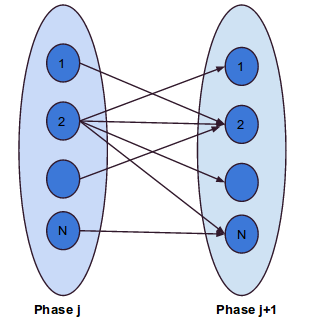
\includegraphics[scale=0.6]{images/ts_table}
  \end{column}
\end{columns}
\end{frame}

\begin{frame}{Algorithm}
\begin{itemize}
\item We divide it in 2 parts-
\item Step 1: Construction of Transition table (Step of Local Optimization)
\item Step 2: Finding the most optimum cycle (Step of Global Optimization)
\end{itemize}
\end{frame}

\begin{frame}{Construction of Transition Table}
\begin{itemize}
\item Consider following transition: \\
    \[\{1\}\{2, 3\}\{4\}, i\] \[\{1,2\}\{3\}\{4\}, i+1\]
\item We know utilization of every virtual machine and hence SUV
\item To find ISUV, we have to find the VMs which are migrating
\item To maximize the profit, we will choose the VM migrations which leads to most profit
\item Because we don't have explicit PM numbering, we have to consider all possible numberings of PMs
\item Fix numbering of PMs in one state\\
\[1-\{1\} 2-\{2,3\} 3-\{4\}, i\]
\item Consider all possible numberings in other state $3! = 6$
\item Choose the one with maximum profit
\end{itemize}
\end{frame}

\begin{frame}{Local Optimization}
\begin{figure}
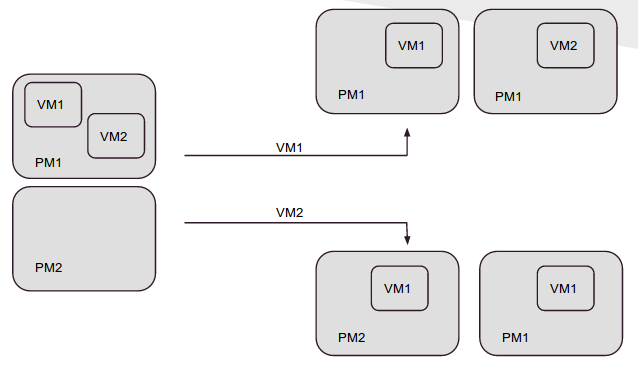
\includegraphics[scale=0.5]{images/lo}
\end{figure}
\end{frame}

\begin{frame}{Global Optimization}
\begin{figure}
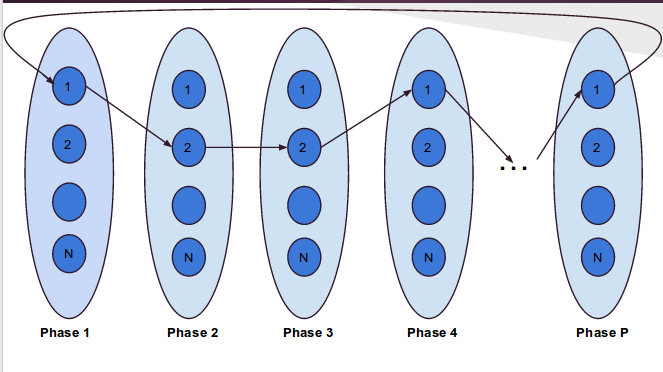
\includegraphics[scale=0.5]{images/go}
\end{figure}
\end{frame}

\begin{frame}{Global Optimization}
\begin{itemize}
\item We choose the start state (and the end state)
\item N such possibilities
\item Max Profit of Cycle beginning at $(S_1, P_1)$:
\item Max Profit from $(S_1, P_1)$ to $(S_k, P_3)$ + Max profit from $(S_k, P_3)$ to $(S_1, P_1)$
\item Max profit from $(S_1, P_1)$ to $(S_k, P_3$: max profit path among all possible paths
\item At the end, we choose the start state with the maximum profit
\end{itemize}
\end{frame}

\begin{frame}{Global Optimization}
\begin{figure}
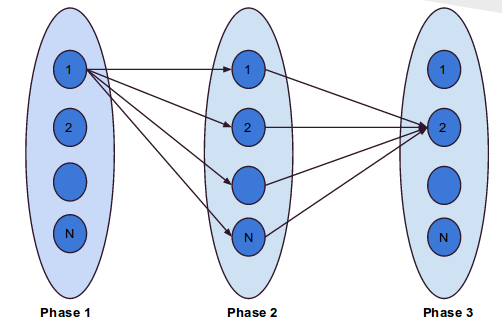
\includegraphics[scale=0.5]{images/go0}
\end{figure}
\end{frame}

\begin{frame}{Global Optimization}
\begin{figure}
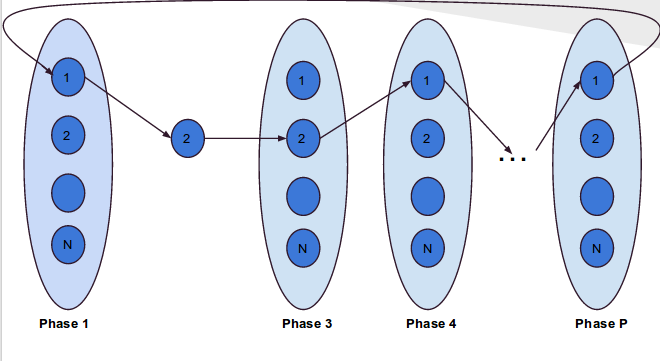
\includegraphics[scale=0.5]{images/go1}
\end{figure}
\end{frame}

\begin{frame}{Global Optimization}
\begin{figure}
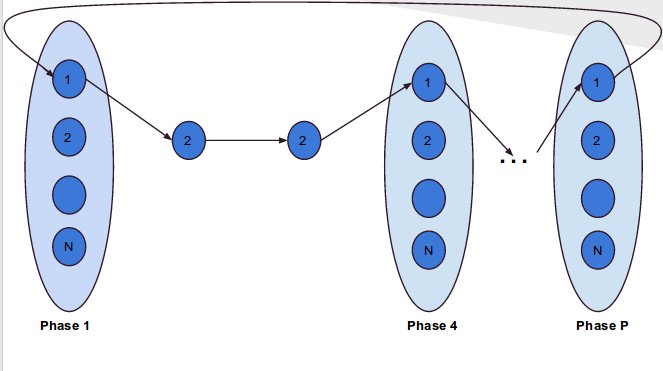
\includegraphics[scale=0.5]{images/go2}
\end{figure}
\end{frame}

\begin{frame}{Global Optimization}
\begin{figure}
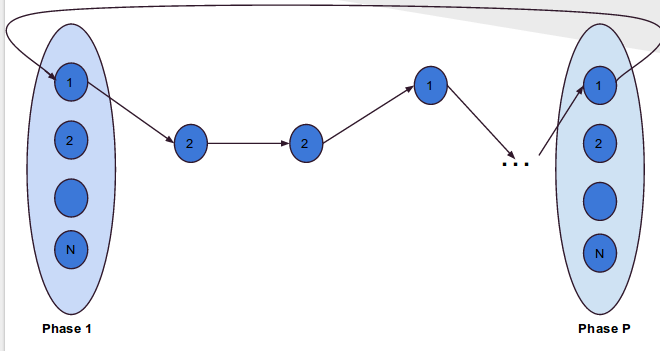
\includegraphics[scale=0.5]{images/go3}
\end{figure}
\end{frame}

\begin{frame}{Asymptotic Complexity}
\begin{itemize}
\item N  $< \left(\frac{0.79N_V}{\log N_V}\right)^{N_V}$
\item Order of N: O$\left(\frac{N_V}{\log N_V}\right) ^{N_V}$
\item Time Complexity: \\
$O\left(N_P*N^{2}*N_V! + \left(N_P-1\right)*N^{3}\right)$
\item Space Complexity : \\
		$O\left(N_P*N^{2}*N_V + N_P*N^{2}\right)$
\end{itemize}
\end{frame}

\section{Results}
\begin{frame}{Results}
\addtocounter{framenumber}{-1}
\tableofcontents[currentsection]
\end{frame}

\section{Resources}
\begin{frame}{Resources}
\begin{itemize}
\item The code is hosted on  \href{https://github.com/mangalaman93/simcon}{github}
\item \href{https://docs.google.com/spreadsheet/ccc?key=0Aoq3-tdSgQ83dGEzakJoUk9pYjlmSXVNN3p1bGtwLWc}{Spreadsheet} containing results
\end{itemize}
\end{frame}


\section{References}
\multipleframe
\begin{frame}[allowframebreaks]
\frametitle{References}
\begin{thebibliography}{9}
\bibitem{khanna}
    \textsc{G. Khanna, K. Beaty, G. Kaur and A. Kochut}, "Application performance management in virtualized data centers" in \textit{Proceedings of the 7th international conference on Autonomic computing}, 2010
\bibitem{vmanage}
    \textsc{S. Kumar, V. Talwar, V. Kumar, P. Ranganathan and K. Schwan}, "vmanage: loosely coupled platform and virtualization management in data centers" in \textit{Proceedings of the 6th international conference on Autonomic computing}, 2009
\bibitem{pmapper}
    \textsc{A. verma, P. Ahuja and A. Neogi}, "pmapper: power and migration cost aware application placement in virtualized systems" in \textit{Proceedings of the 9th ACM/IFIP/USENIX international conference on middleware}, 2008
\bibitem{mdp}
    \textsc{T. Satish, Varsh Apte}, "long term profit sensitive server consolidation", \textit{M.Tech Dissertion report} IIT Bombay, 2013
\bibitem{knuth}
    \textsc{Donald E. Knuth}, "The art of computer programming" http://www.cs.utsa.edu/~wagner/knuth/fasc3b.pdf
\bibitem{bell}
    \textsc{Wikipedia}, "Sterling number of second kind"
\bibitem{permut}
    \textsc{HackerEarth}, "Permutation of N numbers" http://learn.hackerearth.com/tutorial/number-theory/14/permutations-of-n-numbers/
\end{thebibliography}
\end{frame}
\restoreframe

\begin{frame} \frametitle{Thank you}
\Huge{\centerline{\color{theme_color}Questions?}}
\end{frame}

\end{document}
